% Diagram for the report (usecase). Build: see build.sh in this folder.
\documentclass[12pt]{standalone}
% Shared style of every diagram and chart in the report.
% Each agent keeps the same colour in every figure.
% The diagrams are drawn here, not in main.tex, so the report itself does not
% load TikZ: it includes the built PDFs and compiles within Overleaf's time limit.
\usepackage{amsmath,amssymb}
\usepackage{xcolor}
\usepackage{tikz}
\usetikzlibrary{positioning,arrows.meta,shapes.geometric,shapes.misc,fit,calc,backgrounds}
\usepackage{pgfplots}
\pgfplotsset{compat=1.18}

% Same text width as the report (A4, 30 mm + 20 mm margins), for the charts.
\setlength{\textwidth}{160mm}
\newcommand{\Rs}{Rs.\,}
\newcommand{\code}[1]{\texttt{\detokenize{#1}}}

\definecolor{ink}{HTML}{2B2B2B}
\definecolor{agAfill}{HTML}{E4F2E1}\definecolor{agAline}{HTML}{3E7D3A} % Agent 1 Document & Vendor
\definecolor{agBfill}{HTML}{FCEBD5}\definecolor{agBline}{HTML}{B8701D} % Agent 2 Approval & Inventory
\definecolor{agCfill}{HTML}{EEE4F4}\definecolor{agCline}{HTML}{6E4A8E} % Agent 3 Contract & Risk
\definecolor{agDfill}{HTML}{FBE4E4}\definecolor{agDline}{HTML}{A8474B} % Agent 4 Platform
\definecolor{infill}{HTML}{E8EDF6}\definecolor{inline}{HTML}{4F6188}    % infrastructure / data
\definecolor{exfill}{HTML}{F2F2F2}\definecolor{exline}{HTML}{6F6F6F}    % people and external systems
\definecolor{humfill}{HTML}{FFF6D6}\definecolor{humline}{HTML}{9A7B12}  % human decision points
\definecolor{chartA}{HTML}{9AA5B1}\definecolor{chartB}{HTML}{3F5E8C}    % chart: baseline / shipped

\tikzset{
  >={Stealth[length=2mm]},
  every picture/.style={font=\footnotesize, line width=0.6pt, draw=ink, text=ink},
  nohyph/.style={execute at begin node={\hyphenpenalty=10000\exhyphenpenalty=10000}},
  box/.style={nohyph, draw, rounded corners=2pt, align=center, inner sep=3pt, minimum height=8mm},
  agA/.style={box, fill=agAfill, draw=agAline},
  agB/.style={box, fill=agBfill, draw=agBline},
  agC/.style={box, fill=agCfill, draw=agCline},
  agD/.style={box, fill=agDfill, draw=agDline},
  infra/.style={box, fill=infill, draw=inline},
  ext/.style={box, fill=exfill, draw=exline},
  human/.style={box, fill=humfill, draw=humline},
  decision/.style={nohyph, diamond, aspect=2.2, draw=humline, fill=humfill, align=center, inner sep=1pt},
  flow/.style={->, draw=ink},
  dflow/.style={->, draw=ink, dashed},
  lbl/.style={font=\scriptsize\itshape, fill=white, inner sep=1pt},
  note/.style={font=\scriptsize\itshape, align=center},
}
\pgfplotsset{
  reportbars/.style={
    ybar, width=0.95\textwidth, height=6cm, ymin=0,
    enlarge x limits=0.18, bar width=11pt,
    ymajorgrids, grid style={draw=black!12},
    axis line style={draw=black!60}, tick style={draw=black!60},
    legend style={draw=none, font=\footnotesize, legend columns=-1, at={(0.5,1.03)}, anchor=south},
    tick label style={font=\footnotesize}, label style={font=\footnotesize},
    nodes near coords, every node near coord/.append style={font=\scriptsize},
    /tikz/every even column/.append style={column sep=0.6cm},
    legend image code/.code={\draw[#1, draw=none] (0cm,-0.1cm) rectangle (0.3cm,0.1cm);},
  },
}

\begin{document}
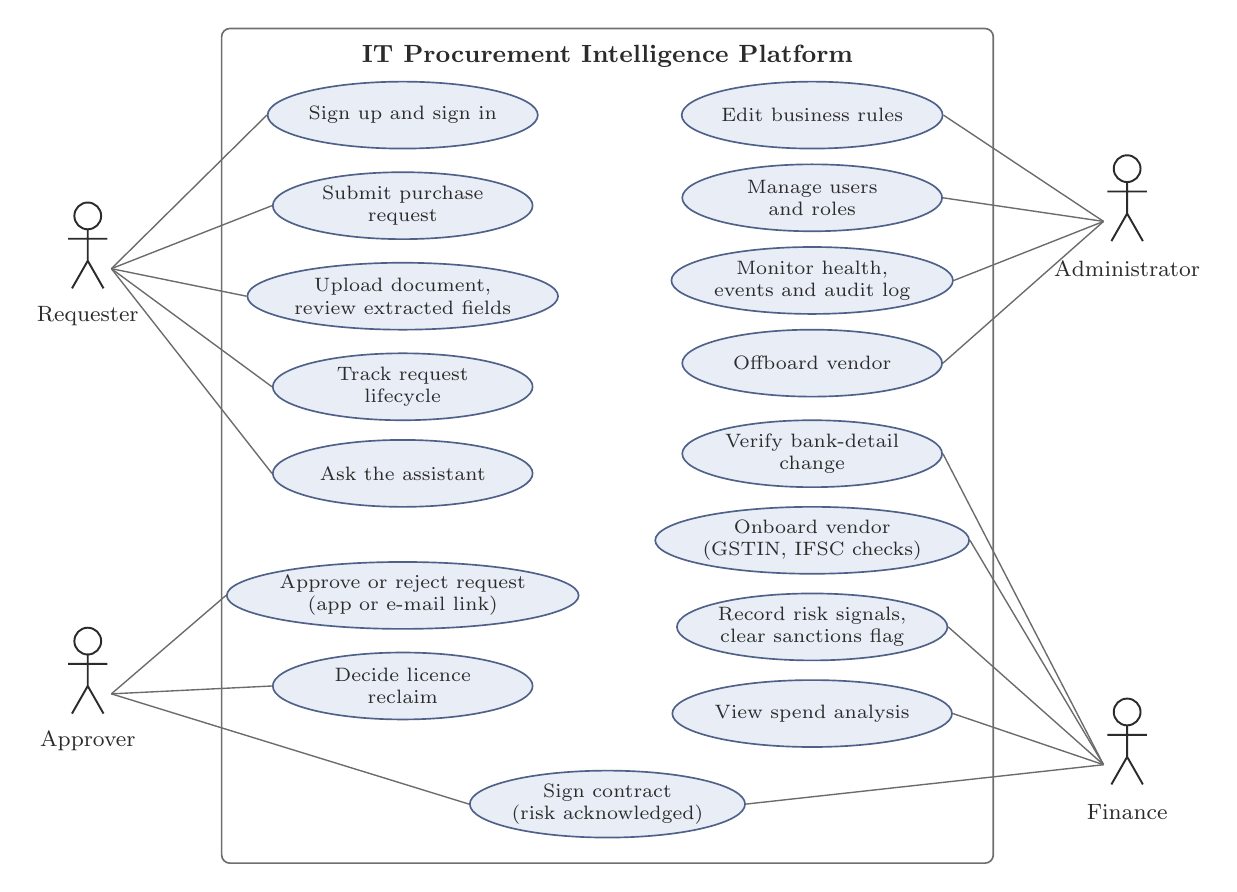
\begin{tikzpicture}
\tikzset{
  uc/.style={nohyph, ellipse, draw=inline, fill=infill, align=center, inner sep=0.5pt, minimum height=8.5mm, minimum width=3.3cm, font=\scriptsize},
  actor/.pic={\draw[line width=0.7pt] (0,0.62) circle (0.17) (0,0.45)--(0,0.05) (-0.25,0.33)--(0.25,0.33) (0,0.05)--(-0.2,-0.3) (0,0.05)--(0.2,-0.3);},
  link/.style={draw=ink!70, line width=0.5pt},
}
\draw[rounded corners=3pt, draw=exline] (-4.9,-5.6) rectangle (4.9,5.0);
\node[font=\small\bfseries] at (0,4.65) {IT Procurement Intelligence Platform};
\pic at (-6.6,2.0) {actor};  \node[font=\footnotesize] at (-6.6,1.35) {Requester};
\pic at (-6.6,-3.4) {actor}; \node[font=\footnotesize] at (-6.6,-4.05) {Approver};
\pic at (6.6,2.6) {actor};   \node[font=\footnotesize] at (6.6,1.95) {Administrator};
\pic at (6.6,-4.3) {actor};  \node[font=\footnotesize] at (6.6,-4.95) {Finance};
\node[uc] (u1) at (-2.6,3.9) {Sign up and sign in};
\node[uc] (u2) at (-2.6,2.75) {Submit purchase\\request};
\node[uc] (u3) at (-2.6,1.6) {Upload document,\\review extracted fields};
\node[uc] (u4) at (-2.6,0.45) {Track request\\lifecycle};
\node[uc] (u5) at (-2.6,-0.65) {Ask the assistant};
\node[uc] (u6) at (-2.6,-2.2) {Approve or reject request\\(app or e-mail link)};
\node[uc] (u7) at (-2.6,-3.35) {Decide licence\\reclaim};
\node[uc] (d1) at (2.6,3.9) {Edit business rules};
\node[uc] (d2) at (2.6,2.85) {Manage users\\and roles};
\node[uc] (d3) at (2.6,1.8) {Monitor health,\\events and audit log};
\node[uc] (d4) at (2.6,0.75) {Offboard vendor};
\node[uc] (f1) at (2.6,-0.4) {Verify bank-detail\\change};
\node[uc] (f2) at (2.6,-1.5) {Onboard vendor\\(GSTIN, IFSC checks)};
\node[uc] (f3) at (2.6,-2.6) {Record risk signals,\\clear sanctions flag};
\node[uc] (f4) at (2.6,-3.7) {View spend analysis};
\node[uc] (u8) at (0,-4.85) {Sign contract\\(risk acknowledged)};
\foreach \u in {u1,u2,u3,u4,u5} \draw[link] (-6.3,1.95) -- (\u.west);
\foreach \u in {u6,u7,u8} \draw[link] (-6.3,-3.45) -- (\u.west);
\foreach \u in {d1,d2,d3,d4} \draw[link] (6.3,2.55) -- (\u.east);
\foreach \u in {f1,f2,f3,f4,u8} \draw[link] (6.3,-4.35) -- (\u.east);
\end{tikzpicture}
\end{document}
